\documentclass[graphics]{beamer}

\usepackage{graphicx}
\usepackage{verbatim}
\usepackage{wrapfig}
\useoutertheme{shadow}
%\usecolortheme{orchid}
\usecolortheme{seahorse}


% math commands
\newcommand{\be}{\begin{eqnarray}}
\newcommand{\ee}{\end{eqnarray}}
\newcommand{\beq}{\begin{equation}}
\newcommand{\eeq}{\end{equation}}
\def\simless{\mathbin{\lower 3pt\hbox
      {$\rlap{\raise 5pt\hbox{$\char'074$}}\mathchar"7218$}}}
\def\simgreat{\mathbin{\lower 3pt\hbox
      {$\rlap{\raise 5pt\hbox{$\char'076$}}\mathchar"7218$}}} %> or of order

% variables

\def\toonscale{0.45}
\def\mboxy#1{\mbox{\small #1}}


\begin{comment}
\AtBeginSection[]{
  \frame{
    \frametitle{Outline}
    \tableofcontents[currentsection]
  }
}
\end{comment}

\title{Fast radio surveys: CHIME and beyond
}
%\subtitle{interim update}
\author[U. Pen]{Ue-Li Pen, CITA/MPIfR
\\[8mm] 
}
\date{November 15, 2019}


\begin{document}

%\section*{Introduction}
\section{Current results}

\begin{comment}
  \subsection{Outline}

  \frame{
    \frametitle{Outline}
    \tableofcontents
  }
\end{comment}

\frame{\maketitle}




  \frame{
\vspace{-0.5in}
    \frametitle{Radio Survey Science}
    \begin{itemize}
        \item FRB
        \item 21cm+IM          
        \item 21cm absorbers
        \item polarization
        \item pulsar search
    \end{itemize}
\vspace{-0.6in}\hspace{2.6in}
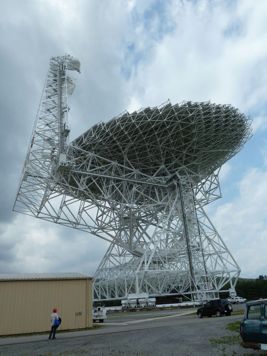
\includegraphics[width=1.5in]{Figures/gbt-eric.png} \vspace{-0.5in}
  }


  \frame{
\vspace{-0.5in}
    \frametitle{Strategy}
    \begin{itemize}
        \item wide FOV
        \item large collecting area
        \item scalable processing cost
        \item FFTT!  ()
        \item 
    \end{itemize}
\vspace{-0.6in}\hspace{2.6in}
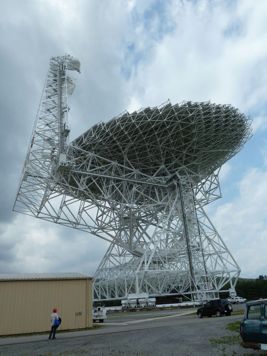
\includegraphics[width=1.5in]{Figures/gbt-eric.png} \vspace{-0.5in}
  }




  \frame{
\vspace{-0.2in}
    \frametitle{map}
\hspace{-0.2in}\includegraphics[width=4.5in]{Figures/sec_A_15hr_41-90_clean_map_I_RADec.mp4}
  }
  \frame{
\vspace{-0.2in}
    \frametitle{residual}
\hspace{-0.2in}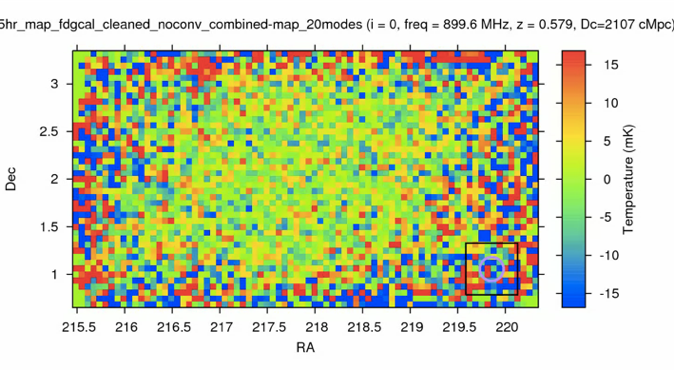
\includegraphics[width=4.5in]{Figures/gbt-residual.png}
  }
  \frame{
    \frametitle{power}
\vspace{-0.2in}
\hspace{-0.3in}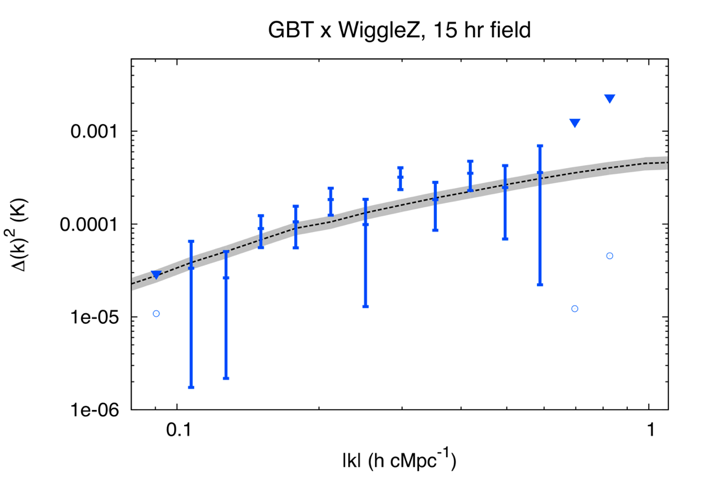
\includegraphics[width=4.5in]{Figures/gbt-power.png}
  }
  \frame{
    \frametitle{Auto power constraints}
%\vspace{-0.2in}
\hspace{-0.1in}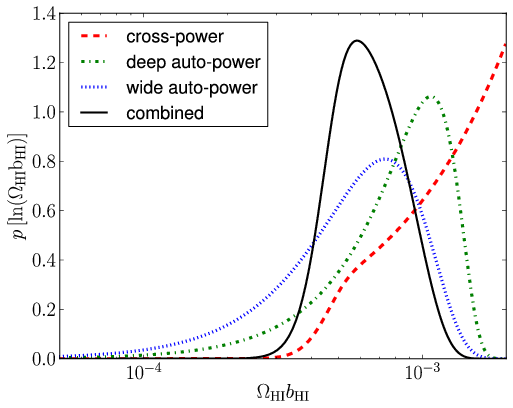
\includegraphics[width=3in]{Figures/gbt-omegahi.png}
Switzer et al 2013
  }

  \frame{
\vspace{-0.5in}
    \frametitle{Parkes-IM}
    \begin{itemize}
      \item 500 beam-hours on 2dF field
      \item measure 21cm $z<0.2$ auto-power, cross-power, RSD, $\Omega_{HI}$
      \item Anderson et al 2018
%          \vspace{-0.15in}
    \end{itemize}
%\vspace{-0.1in}
\hspace{.3in}
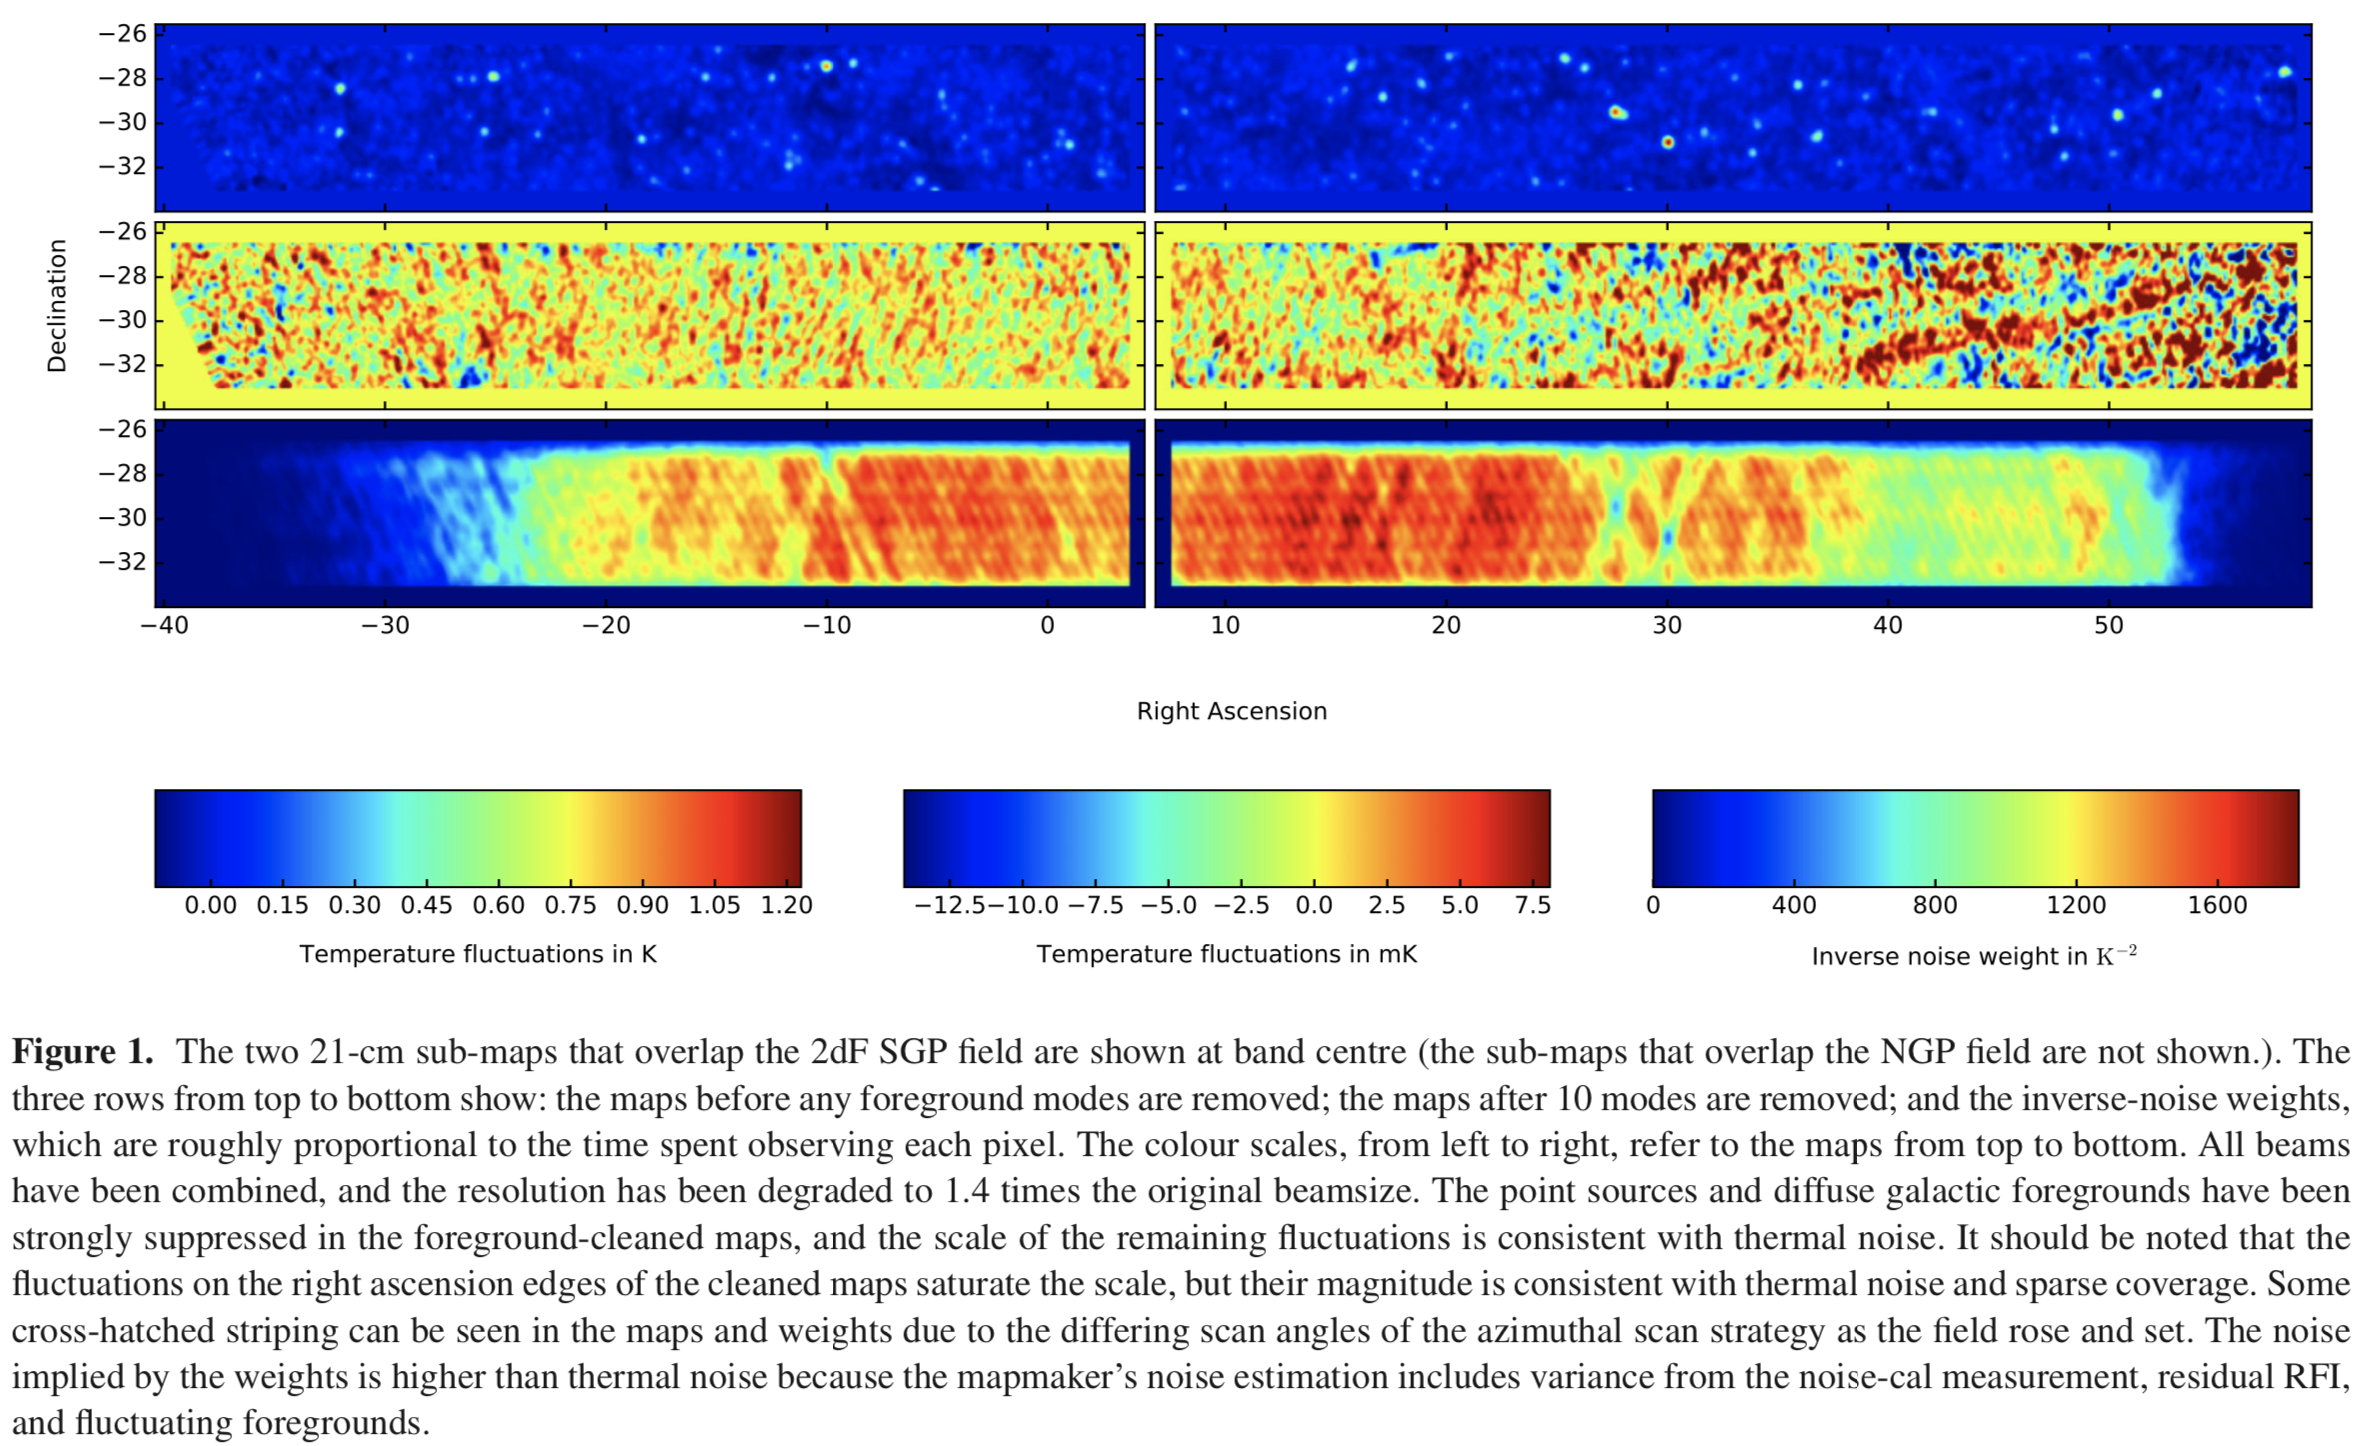
\includegraphics[width=3in]{Figures/parkes.png}\vspace{-0.4in}
  }
  \frame{
    \frametitle{HIPASS comparison}
%\vspace{-0.2in}
\hspace{0.1in}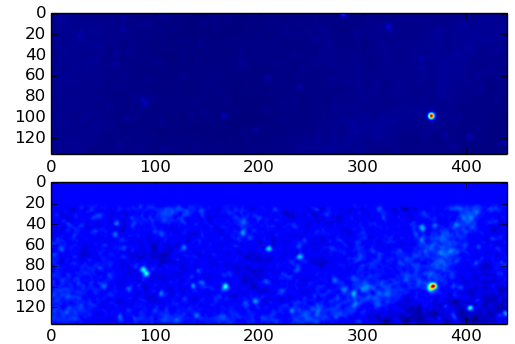
\includegraphics[width=3.5in]{Figures/parkes-ra199crop.png}
  }


  \frame{
    \frametitle{EoR}
    \begin{itemize}
        \item rollercoaster: best constraints get retracted
        \item GMRT-EoR: Paciga et al 2011 -- 2013, longest standing
          upper bound, NSERC SRO funded
        \item PAPER: Parsons et al 2013 -- Cheng et al 2018
        \item LOFAR: Patil et al 2017, update to 2019?
        \item MWA: Beardsley et al 2016 --
    \end{itemize}
}

\section{Ongoing Experiments}
  \frame{
    \frametitle{CHIME}
    \begin{itemize}
        \item CHIME commissioning, first maps
        \item foreground removal: multiple strategies
    \end{itemize}
%\vspace{-0.1in}\hspace{.3in}
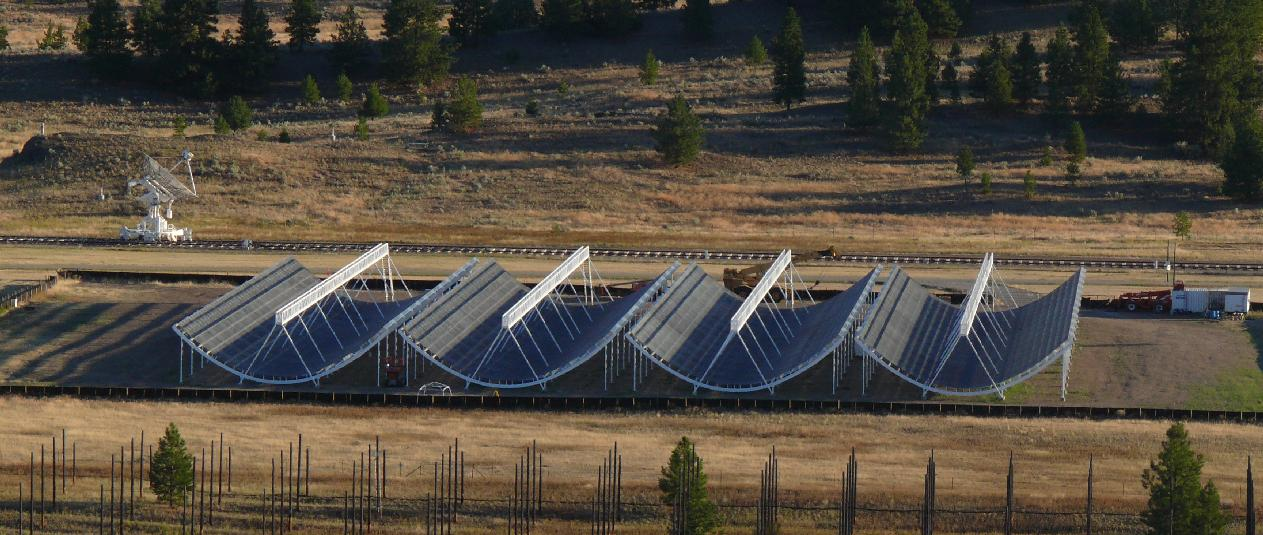
\includegraphics[width=4in]{Figures/Chime-medium.jpg}
}

  \frame{
\vspace{-0.2in}
    \frametitle{MAP}
\hspace{-0.2in}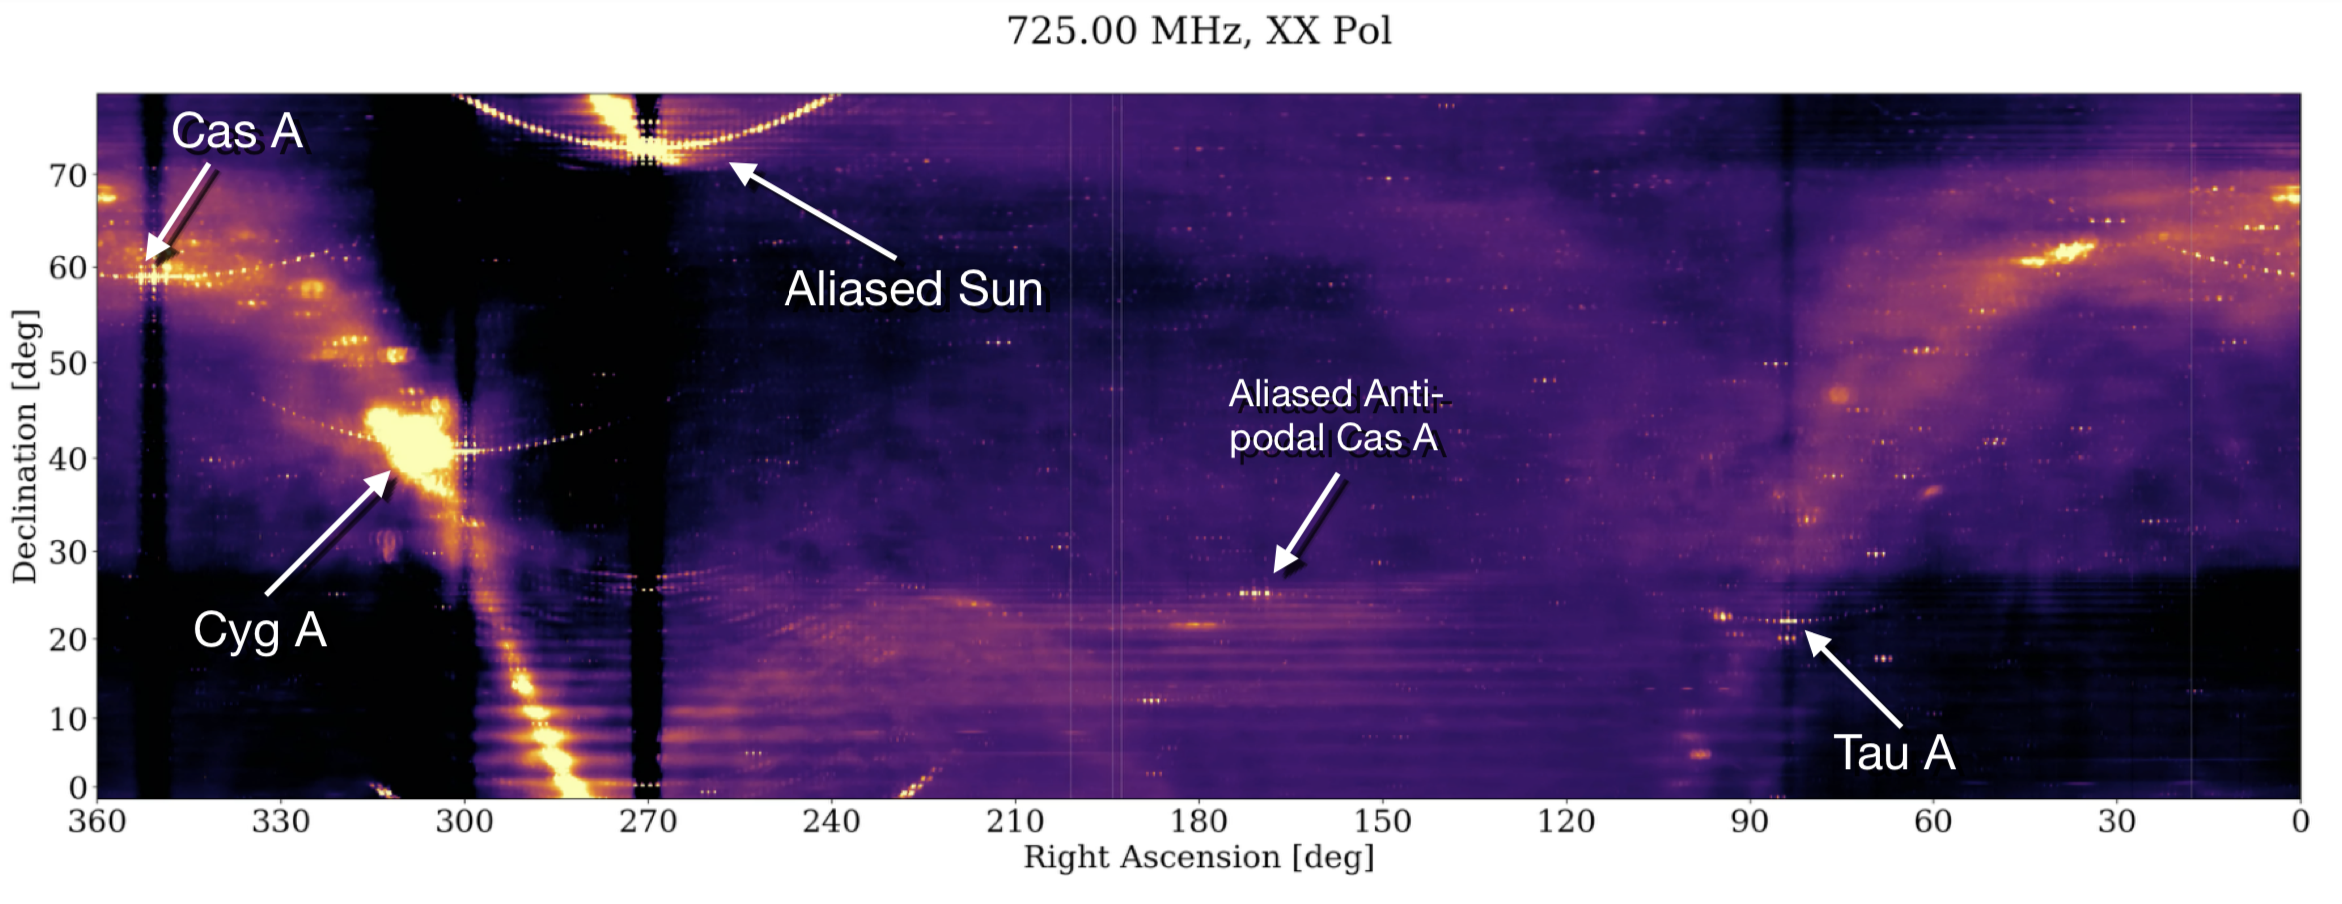
\includegraphics[width=4.5in]{Figures/CHIME-map.png}
  }

  \frame{
    \frametitle{Tianlai}
    \begin{itemize}
        \item in Xinjiang, China
        \item currently commissioning
    \end{itemize}
%\vspace{-0.1in}\hspace{.3in}
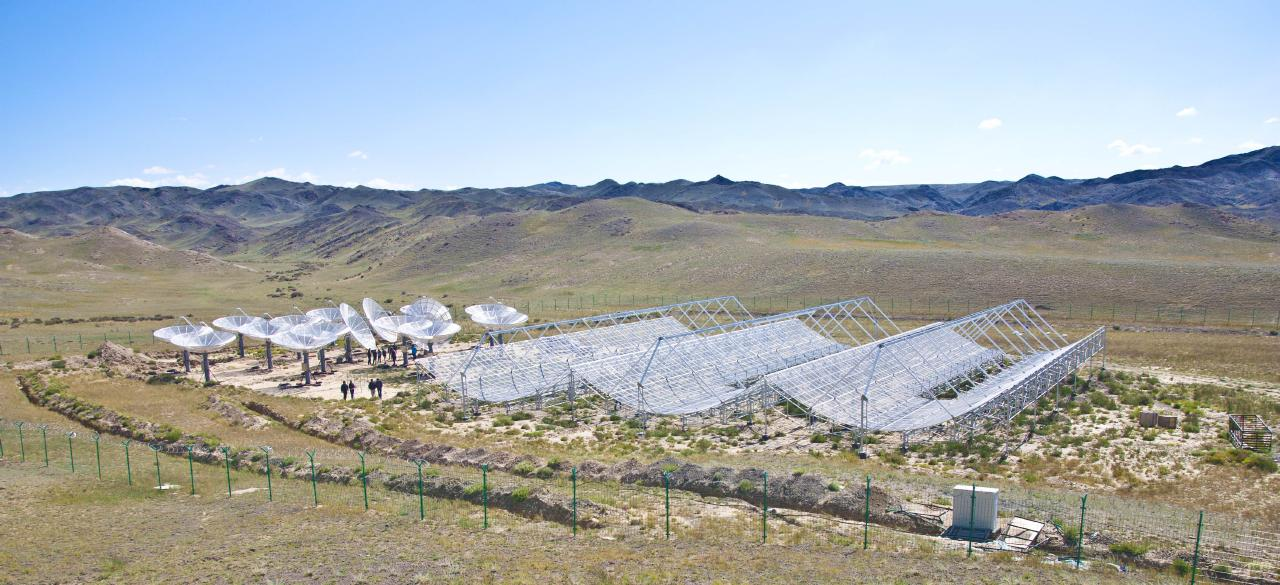
\includegraphics[width=4in]{Figures/tianlai-medium.jpg}
}

  \frame{
    \frametitle{HIRAX}
    \begin{itemize}
        \item Karoo, SA
        \item most ambitious IM-BAO project, doubles as pulsar and FRB engine
    \end{itemize}
%\vspace{-0.1in}\hspace{.3in}
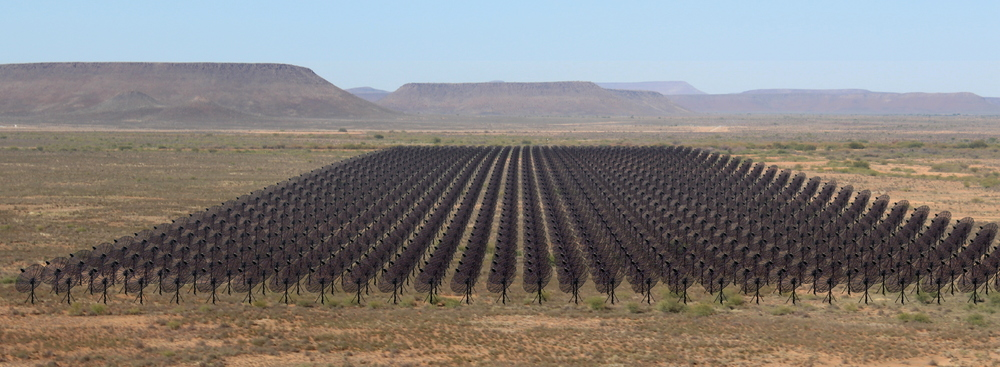
\includegraphics[width=4in]{Figures/hirax-karoo-s.jpg}
}
\section{Lessons learned}
  \frame{
    \frametitle{Observing strategy}
    \begin{itemize}
        \item drift scan: all approaches now utilize drift scans
        \item $m$-mode transform: eliminate E-W mode mixing! (Shaw et
          al 2014, 2015)
        \item scale invariant N-S imaging: apodization to common beam
    \end{itemize}
}


  \frame{
    \frametitle{Outlook}
    \begin{itemize}
        \item 21cm foreground challenge resulted in diverse approaches
        \item biggest achieved removal in single dish GBT: compact
          filled aperture
        \item Canadian leaderhip: CHIME, HIRAX, GBT, GMRT-EoR
    \end{itemize}
}

\end{document}
